\section{Stacking-Probleme}
\label{sec:stacking_problems}

Stacking-Probleme treten in der Praxis zum Beispiel im Umfeld von Lagerhallen und Container-Terminals auf.
Ankommende \textit{Items}, häufig Container, müssen sogenannten \textit{Stacks} zugeordnet werden, sodass bestimmte Nebenbedingungen respektiert werden.
Diese Nebenbedingungen sorgen zum Beispiel dafür, dass nicht jedes \textit{Item} auf jedem anderen \textit{Item} platziert werden
darf. Es wird dabei angenommen, dass die im Folgenden als \textit{Storage-Area} bezeichnete Lagerfläche in festen
\textit{Stacks} organisiert ist, die eine limitierte gemeinsame Höhe besitzen, die im Folgenden als \textit{Stack}-Kapazität bezeichnet wird.\newline
Es kann in der Regel nur auf das oberste \textit{Item} eines \textit{Stacks} zugegriffen werden, d.h. der \textit{Item}-Zugriff erfolgt
nach dem \textquote{Last-In–First-Out}-Prinzip. Ein Zugriff auf \textit{Items} darunter erfordert eine \textit{Relocation}-Operation, die
zeit- und energieaufwendig ist.\newline

In dieser Arbeit wird nur der \textit{Loading}-Prozess betrachtet, währenddem keine \textit{Item}-Entnahme stattfindet.
Die \textit{Items} werden in die \textit{Storage-Area} geladen, die aus \textit{Stacks} mit einer festen Position besteht, d.h.
man kann die \textit{Stacks} nicht positionieren, sondern lediglich den \textit{Items} eine Position in einem \textit{Stack} zuweisen.\newline
Der \textit{Relocation}-Prozess wird typischerweise durch Kräne durchgeführt, die den \textit{Stacks} eine Maximalhöhe auferlegen.

Neben der Tatsache, dass nicht jedes \textit{Item} auf jedem anderen \textit{Item} platziert werden darf, gilt auch, dass es \textit{Items} gibt, die auf bestimmte Positionen beschränkt sind, weil sie zum Beispiel eine Energiequelle benötigen.
Abbildung \ref{fig:storage_area} zeigt den Aufbau der \textit{Storage-Area} bestehend aus $m$ fixierten
\textit{Stacks}, die jeweils $b$ \textit{Level} enthalten. Jedes \textit{Level} innerhalb eines \textit{Stacks} entspricht dabei einer Position, der ein \textit{Item} zugeordnet werden kann.

\begin{figure}[H]
\centering
\resizebox{0.5\textwidth}{!}{
\begin{tabular}{|c|c|c|c|c|c|}
\cline{1-5}
$\boldsymbol{S_1}$ & $\boldsymbol{S_2}$ & $\boldsymbol{S_3}$ & ... & $\boldsymbol{S_m}$\\ \cline{1-5}
\end{tabular}}
\caption*{\textsc{von oben betrachtet}}
\end{figure}
\begin{figure}[H]
\centering
\resizebox{0.5\textwidth}{!}{
\begin{tabular}{c|c|c|c|c|c|}
\cline{2-6}
$\boldsymbol{L_b}$ & $pos_{1, b}$ & $pos_{2, b}$ & $pos_{3, b}$ & ... & $pos_{m, b}$ \\ \cline{2-6}
... & ... & ... & ... & ... & ...\\ \cline{2-6}
$\boldsymbol{L_2}$ & $pos_{1, 2}$ & $pos_{2, 2}$ & $pos_{3, 2}$ & ... & $pos_{m, 2}$\\ \cline{2-6}
$\boldsymbol{L_1}$ & $pos_{1, 1}$ & $pos_{2, 1}$ & $pos_{3, 1}$ & ... & $pos_{m, 1}$\\ \cline{2-6}
\multicolumn{1}{c}{} & \multicolumn{1}{c}{$\boldsymbol{S_1}$} & \multicolumn{1}{c}{$\boldsymbol{S_2}$}
& \multicolumn{1}{c}{$\boldsymbol{S_3}$} & \multicolumn{1}{c}{...} & \multicolumn{1}{c}{$\boldsymbol{S_m}$} \\
\end{tabular}}
\caption*{\textsc{von der Seite betrachtet}}

\caption{\textsc{Aufbau der \textit{Storage-Area}}}
\label{fig:storage_area}
\end{figure}

Das Ziel von Stacking-Problemen ist es, jedes ankommende \textit{Item} einer zulässigen Position in einem
\textit{Stack} zuzuordnen, sodass eine gegebene Zielfunktion optimiert wird. Es gibt eine ganze Reihe praktisch relevanter Zielfunktionen,
in dieser Arbeit geht es um die Minimieren der Transportkosten, die bei der Verladung der \textit{Items} von ihrer Originalposition zur zugewiesenen Stackposition entstehen.

%%%%%%%%%%%%%%%%%%%%%%%%%%%%%%%%%%%%%%%%%%%%%%%%%%%%%%%%%%%%%%%%%%%%%%%%%%%%%%%%%%%%%%%%%%%%%%%%%%%%
\pagebreak
%%%%%%%%%%%%%%%%%%%%%%%%%%%%%%%%%%%%%%%%%%%%%%%%%%%%%%%%%%%%%%%%%%%%%%%%%%%%%%%%%%%%%%%%%%%%%%%%%%%%

\section{Formale Definition}
\label{sec:formal_definition}

Die \textit{Storage-Area} besteht aus \textit{Stacks}, die in einer Reihe angeordnet sind (vgl. Abb. \ref{fig:storage_area}). Die x-Koordinate spezifiziert jeweils den \textit{Stack} und die y-Koordinate den \textit{Level} innerhalb des jeweiligen \textit{Stacks}. Es handelt sich also um eine Reihe von $m$ \textit{Stacks} mit jeweils $b$ Positionen pro \textit{Stack}. Abb. \ref{fig:parameters} zeigt eine Liste der
Parameter, die im weiteren Verlauf der Arbeit immer wieder verwendet werden, um Stacking-Probleme zu definieren.
\begin{figure}[H]
\centering
\resizebox{0.5\textwidth}{!}{
\begin{tabular}{ | l | l |}
    \hline
    \textbf{Parameter} & \textbf{Semantik} \\ \hline
    $n$ & Anzahl der Items \\ \hline
    $m$ & Anzahl der Stacks \\ \hline
    $b$ & Stack Kapazität \\ \hline
    $I$ & Menge der Items $ I := \{1, 2, ..., n\}$ \\ \hline
\end{tabular}}
\caption{\textsc{Zur Definition verwendete Parameter}}
\label{fig:parameters}
\end{figure}
In der Regel gilt $m < n$, d.h. es müssen \textit{Items} gestapelt werden.
Außerdem muss die Annahme $n \leq bm$ gelten, denn sonst ist die Instanz des Problems unzulässig,
weil es mehr \textit{Items} als Positionen gibt.\newline
Für jedes \textit{Item} $i \in I$ ist dessen Originalposition $O_i$ in x- und y-Koordinaten gegeben.

\textit{Items}, die in einem \textit{Stack} platziert werden, sind durch ein Tupel $(i_k, ..., i_1)$ definiert, wobei
$i_\lambda$ das \textit{Item} auf \textit{Level} $\lambda$ beschreibt. $\lambda = 1$ beschreibt den \textit{Ground-Level}.
Instanzen können Stacking-Restriktionen $s_{ij}$ enthalten, die angeben, ob ein \textit{Item} $i$ direkt auf einem \textit{Item} $j$ platziert
werden darf. Dies ist der Fall, wenn $s_{ij} = 1$ gilt.
Ein Tupel ist zulässig, wenn $k \leq b$ und $s_{i_{\lambda + 1}, i_\lambda} = 1 \quad \forall \quad \lambda = 1, ..., k - 1$.
D.h. ein Tupel ist dann zulässig, wenn die \textit{Stack}-Kapazität eingehalten wird und alle \textit{Items}, die aufeinander gestapelt sind,
nicht den Stacking-Restriktionen widersprechen, die in Kapitel \ref{stacking_restrictions} erläutert werden.

\textbf{Formulierung des Problems}\newline
Gegeben sei eine Menge $I = \{1, ..., n\}$ von \textit{Items} und eine Menge $Q = \{1, ..., m\}$ von \textit{Stacks} mit einer \textit{Stack}-Kapazität von $b$. Außerdem seien \textit{Stacking Constraints} $s_{ij}$ und \textit{Placement Constraints} $t_{iq}$ gegeben.
Das Ziel ist nun, jedes \textit{Item} $i \in I$ genau einem \textit{Stack} $q \in Q$ zuzuweisen, wobei die \textit{Stacking Constraints} $s_{ij}$,
die Placement Constraints $t_{iq}$ und die Stack-Kapazität $b$ respektiert werden und gegebenenfalls eine Zielfunktion optimiert wird.

%%%%%%%%%%%%%%%%%%%%%%%%%%%%%%%%%%%%%%%%%%%%%%%%%%%%%%%%%%%%%%%%%%%%%%%%%%%%%%%%%%%%%%%%%%%%%%%%%%%%
\pagebreak
%%%%%%%%%%%%%%%%%%%%%%%%%%%%%%%%%%%%%%%%%%%%%%%%%%%%%%%%%%%%%%%%%%%%%%%%%%%%%%%%%%%%%%%%%%%%%%%%%%%%

\section{Nebenbedingungen}
\label{sec:constraints}

\subsection{Stacking Restriktionen}
\label{sec:stacking_restrictions}

Es gibt in der Praxis vielfältige Gründe dafür, dass nicht jedes \textit{Item} auf jedes andere \textit{Item} gestapelt werden darf.
Aus diesen resultieren bestimmte Restriktionen, die z.B. wie folgt lauten:
\begin{itemize}
  \item schwerere \textit{Items} dürfen nicht auf leichteren \textit{Items} platziert werden
  \item längere \textit{Items} dürfen nicht auf kürzeren \textit{Items} platziert werden
  \item \textit{Items} bestimmter Materialien oder Zielorte dürfen nicht aufeinander gestapelt werden
\end{itemize}

All jene Restriktionen, die im Folgenden stets als \textit{Stacking Constraints} bezeichnet werden, werden in einer Binärmatrix $S = (s_{ij})_{n \times n}$ kodiert, wobei:
\[
    s_{ij} =
\begin{cases}
    1, & \text{wenn $i$ direkt auf $j$ gestapelt werden darf }\\
    0, & \text{sonst}
\end{cases}
\]
Diese Matrix lässt sich, wie in Abb. \ref{fig:matrix_to_graph} beispielhaft dargestellt,
als gerichteter Graph mit $n$ Knoten und Kanten $i \rightarrow j$ für alle $s_{ij} = 1$ repräsentieren.
\begin{figure}[H]
  \begin{subfigure}[b]{0.5\textwidth}
  \centering
    $S =$
    $\left(
    \begin{array}{rrrr}
    0 & 1 & 1 & 0 \\
    1 & 0 & 1 & 0 \\
    1 & 0 & 0 & 0 \\
    1 & 1 & 1 & 0 \\
    \end{array} \right) $
    \caption{\textsc{Constraint Matrix}}
    \label{fig:constraint_matrix}
  \end{subfigure}
  \hfill
  \begin{subfigure}[b]{0.5\textwidth}
  \centering
    \begin{tikzpicture}[->, scale=0.50, transform shape, node distance=2.5cm]
    \node[state] (A) {1};
    \node[state] (B) [right of=A] {2};
    \node[state] (C) [below of=A] {3};
    \node[state] (D) [right of=C] {4};

    \path (A) edge node {} (B)
          (A) edge node {} (C)

          (B) edge [bend right] node {} (A)
          (B) edge [bend left=10] node {} (C)

          (C) edge [bend left] node {} (A)

          (D) edge [bend left=10] node {} (A)
          (D) edge node {} (B)
          (D) edge node {} (C);
  \end{tikzpicture}
    \caption{\textsc{Resultierender Graph}}
    \label{fig:resulting_graph}
  \end{subfigure}
  \caption{\textsc{Stacking Constraints interpretiert als Matrix bzw. Graph.}}
  \label{fig:matrix_to_graph}
\end{figure}
\textit{Stacking Constraints} können transitiv sein. Ist dies der Fall, so gilt folgendes:\newline
Wenn \textit{Item} $i$ auf \textit{Item} $j$ und \textit{Item} $j$ auf \textit{Item} $h$ gestapelt werden darf,
so darf auch \textit{Item} $i$ auf \textit{Item} $h$ gestapelt werden.\newline
Restriktionen bezüglich des Gewichts und der Länge haben die besondere Eigenschaft, dass alle Items vergleichbar sind, d.h. für alle $i \neq j  \quad \text{gilt} \quad s_{ij} = 1 \quad \text{oder} \quad s_{ji} = 1$, was bedeutet, dass diese Restriktionen eine totale Ordnung auf allen \textit{Items} definieren.

%%%%%%%%%%%%%%%%%%%%%%%%%%%%%%%%%%%%%%%%%%%%%%%%%%%%%%%%%%%%%%%%%%%%%%%%%%%%%%%%%%%%%%%%%%%%%%%%%%%%
\pagebreak
%%%%%%%%%%%%%%%%%%%%%%%%%%%%%%%%%%%%%%%%%%%%%%%%%%%%%%%%%%%%%%%%%%%%%%%%%%%%%%%%%%%%%%%%%%%%%%%%%%%%

\section{Das Zulässigkeitsproblem}
\label{decision_problem}

Die simpelste Variante des Storage Loading Problems ist ein Zulässigkeitsproblem, welches die Frage stellt, ob sämtliche Items der Storage Area zugewiesen werden können, sodass alle Nebenbedingungen respektiert werden.
Diese Nebenbedingungen beziehen sich z.B. auf die Stack Kapazität, die Stacking Constraints, ein Gewichtslimit pro Stack oder auch
Restriktionen bezüglich der Position.\newline
Sollte dies möglich sein, so ist häufig das Ziel, jedes Item einer zulässigen Position zuzuweisen.
Diese Position zeichnet sich durch einen Stack-Index und einen Level innerhalb des Stacks aus.
Dabei kann z.B. eine der in Abb. \ref{fig:objective_functions} dargestellten Zielfunktionen optimiert werden, was jedoch bereits über
das Zulässigkeitsproblem hinausgeht.

\pagebreak

\textbf{Exkurs: Maximum-Cardinality-Matching (MCM)}\newline
Gegeben sei ein ungerichteter Graph $G = (V, E)$. Eine Menge $M \subseteq E$ heißt Matching,
wenn keine zwei Kanten aus $M$ einen Knoten gemeinsam haben. Falls $M$ als Menge eine maximale Kardinalität unter
allen Matchings von $G$ hat, wird dies als Maximum-Cardinality-Matching bezeichnet. \cite{WikiMatching}
Es kann mehrere unterschiedliche MCMs in einem Graphen geben.
In Abb. \ref{fig:mcm_examples} werden beispielhaft zwei MCMs dargestellt.
\begin{figure}[H]
  \begin{subfigure}[b]{0.4\textwidth}
  \centering
    \begin{tikzpicture}[scale=0.45, transform shape, node distance=2cm]
    \node[state] (A) {};
    \node[state] (B) [above right of=A] {};
    \node[state] (C) [below left of=A] {};
    \node[state] (D) [below right of=C] {};
    \node[state] (F) [below right of=B] {};
    \node[state] (E) [below of=F] {};

    \path (A) edge [red] node {} (B)
          (A) edge node {} (C)
          (A) edge node {} (D)
          (A) edge node {} (E)
          (A) edge node {} (F)
          (C) edge [red] node {} (D);
  \end{tikzpicture}
  \caption{\textsc{$|MCM| = 2$}}
  \label{fig:mcm1}
  \end{subfigure}
  \hfill
  \begin{subfigure}[b]{0.4\textwidth}
  \centering
    \begin{tikzpicture}[scale=0.45, transform shape, node distance=2cm]
    \node[state] (A) {};
    \node[state] (B) [right of=A] {};
    \node[state] (C) [right of=B] {};
    \node[state] (D) [below left of=A] {};
    \node[state] (E) [below right of=D] {};
    \node[state] (F) [right of=E] {};

    \path (A) edge node {} (B)
          (B) edge [red] node {} (C)
          (B) edge node {} (F)
          (A) edge node {} (E)
          (E) edge [red] node {} (F)
          (A) edge [red] node {} (D)
          (D) edge node {} (E);
  \end{tikzpicture}
    \caption{\textsc{$|MCM| = 3$}}
    \label{fig:mcm_2}
  \end{subfigure}
  \caption{\textsc{Zwei Beispiele für MCMs (dargestellt in rot).}}
  \label{fig:mcm_examples}
\end{figure}

\pagebreak

\textbf{Exkurs: Minimum-Weight-Perfect-Matching}\newline
Zunächst einmal ist es wichtig, zu erwähnen, dass ein Perfect-Matching nur für Graphen mit einer geraden Anzahl an Knoten möglich ist.
Ein Perfect-Matching ist ein Matching, welches sämtliche Knoten des Graphen matcht.
D.h. jeder Knoten des Graphen ist inzident zu genau einer Kante des Matchings (vgl. Abb. \ref{fig:perfect_matching}).
Ein Minimum-Weight-Perfect-Matching ist nun ein günstigstes Perfect-Matching basierend auf den Kantenkosten.
\begin{figure}[H]
\centering
\begin{tikzpicture}[-, scale=0.40, transform shape, node distance=3cm]
    \node[state] (A) {};
    \node[state] (B) [above right of=A] {};
    \node[state] (C) [below right of=A] {};
    \node[state] (D) [right of=B] {};
    \node[state] (E) [right of=D] {};
    \node[state] (F) [right of=C] {};

    \path (A) edge [red] node {} (B)
          (A) edge node {} (C)
          (B) edge node {} (D)
          (B) edge node {} (C)
          (D) edge [red] node {} (E)
          (D) edge node {} (F)
          (C) edge [red] node {} (F);
\end{tikzpicture}
\caption{\textsc{Beispiel für ein Perfect-Matching (rot).}}
\label{fig:perfect_matching}
\end{figure}

\pagebreak

\textbf{Exkurs: Bipartiter Graph}\newline
Ein Graph $G = (V, E)$ heißt bipartit (vgl. Abb. \ref{fig:bipartite_graph}), wenn die Knotenmenge in zwei disjunkte Teilmengen zerfällt
$(V = S \cup T$ mit $S \cap T = \emptyset$), sodass jede Kante einen Knoten aus $S$ mit einem Knoten aus $T$ verbindet. \cite{HochschuleDarmstadt}\newline
Es lassen sich folgende Äquivalenzen festhalten:
\begin{itemize}
  \item $G$ bipartit $\iff$ $G$ 2-färbbar
  \item $G$ bipartit $\iff$ keine Kreise ungerader Länge in $G$
\end{itemize}

\begin{figure}[H]
\centering
\begin{tikzpicture}[scale=0.50, transform shape, node distance=3cm]
  \node[state] [green] (A) {};
  \node[state] [red] (B) [above right of=A] {};
  \node[state] [green] (C) [below right of=B] {};
  \node[state] [red] (D) [below of=B] {};
  \node[state] [red] (E) [below of=A] {};
  \node[state] [green] (F) [right of=E] {};

  \path (A) edge node {} (B)
        (B) edge node {} (C)
        (C) edge node {} (D)
        (A) edge node {} (D)
        (A) edge node {} (E)
        (E) edge node {} (F)
        (D) edge node {} (F);

\end{tikzpicture}
\caption{\textsc{Bipartiter Graph.}}
\label{fig:bipartite_graph}
\end{figure}

\pagebreak

\subsection{Literatur zitieren}

Mit dem \texttt{\textbackslash{}cite} Befehl sieht es folgenderma"sen aus:
\cite{Lehnfeld2014}.

Mit dem Befehl \texttt{\textbackslash{}citet} bzw. \texttt{\textbackslash{}textcite} stattdessen so:
\textcite{Lehnfeld2014}.

Wenn nur die Namen der Autoren benötigt werden, kann
\texttt{\textbackslash{}citeauthor} benutzt werden: \citeauthor{Lehnfeld2014}.

Und hier noch ein Buch \cite{Brucker2007} und ein Konferenzartikel
\cite{Huang2010}.

\subsection{Gleichungen referenzieren}
\label{sec:gleichungen-referenzieren}

Die folgende Gleichung hat das Label \texttt{eq:polyederformel}.
Somit kann sie, wie alle anderen gelabelten Objekte, mit
\texttt{\textbackslash{}ref\{eq:polyederformel\}}
referenziert werden.
Mit dem Befehl \texttt{\textbackslash{}eqref}
erh"alt man die Referenz in runden Klammern:
Gleichung~\eqref{eq:polyederformel}.

\begin{equation}
  \label{eq:polyederformel}
  E - K + F = 2
\end{equation}

Sei $x \in \mathbb{R}$. Nun betrachte die Summe $\sum_{i=1}^n \sum_{\ell = 0}^{i} x^\ell$ ... und folgende Gleichungen
% Gleichungen mit alignment, jeweils mit und ohne Numerierung
\begin{align}
a &= b + c + d      \label{eqn:important1} \\
  &= b + c + e - f  \nonumber \\
  &= xy             \label{eqn:important2}
\end{align}

Aus Gleichungen \eqref{eqn:important1} und \eqref{eqn:important2} folgt ...

\begin{mytheorem}
	Dies ist ein Theorem.
\end{mytheorem}
\begin{proof}
	Dies ist ein Beweis.
\end{proof}

\subsection{LP-Formulierung}
\label{subsec:lp}

\begin{align}
\max 	&& \sum_{i = 1}^n c_i x_i \label{eq:zielf}\\
\text{s.t.} && \sum_{i = 1}^n w_i x_i &\leq W&& \label{eq:c1}\\
	&& x_i & \in \{0, 1\} && (i = 1, \ldots, n)
\end{align}
In der Zielfunktion \eqref{eq:zielf} wird irgend etwas mininimiert ...



\subsection{Tabellen}

\begin{table}[!htbp] \centering
\small
\begin{tabular}{|r|r||r|r|r||r|r|r||r|r|r||} \hline
& & \multicolumn{3}{c||}{$\alpha=0$} & \multicolumn{3}{c||}{$\alpha=0.5$} & \multicolumn{3}{c||}{$\alpha=0.8$}\\
$m$ & $n$ & \# ver & gap & time &  \# ver & gap & time &  \# ver & gap & time  \\  \hline
2 & 10   & 5  & 0	& 1	& 5 & 0   	& 0	& 5 &0		& 0\\
2 & 50   & 3  & 0.01	& 721	& 3 & 0.01	& 742	& 0 &0.84	& 1800\\
2 & 100  & 4  & 0.00	& 367	& 4 & 0.00	& 491	& 0 &0.35	& 1800\\
2 & 150  & 5  & 0	& 40	& 5 & 0		& 811	& 0 &0.27	& 1800\\
3 & 10   & 5  & 0	& 0	& 5 & 0		& 0	& 5 &0 		& 0\\
3 & 50   & 3  & 0.01	& 1094	& 1 & 0.03	& 1752	& 0 &2.12	& 1800\\
3 & 100  & 5  & 0	& 243	& 0 & 0.22	& 1800	& 0 &2.23	& 1800\\
3 & 150  & 4  & 0.00	& 894	& 0 & 0.15	& 1800	& 0 &3.18	& 1800 \\
5 & 10   & 5  & 0	& 0	& 5 & 0 	& 0	& 5 &0 		& 0 \\
5 & 50   & 1  & 0.02	& 1669	& 0 & 0.98	& 1800	& 0 &8.35 	& 1800\\
5 & 100  & 1  & 0.02	& 1785	& 0 & 1.15	& 1800	& 0 &8.38 	& 1800 \\
5 & 150  & 0  & 0.04	& 1800	& 0 & 1.18	& 1800	& 0 &10.59 	& 1800 \\ \hline
\multicolumn{2}{l||}{\ }  &
           41  &0.01	& 717	&28 & 0.31	& 1066	& 15 &3.03 	& 1350
\end{tabular}
\caption{Ergebnisse f"ur das MIP.}
    \label{tab:mip_lb}
\end{table}


\subsection{Ein Algorithmus}
\label{sec:algorithmus}

\SetKwInOut{Parameter}{parameter}

\begin{algorithm}[ht]
\SetKwData{Left}{left}
\SetKwData{This}{this}
\SetKwData{Sink}{$a'$}
\SetKwFunction{Sleep}{Sleep}
\SetKwFunction{Append}{Append}

\SetKwInOut{Input}{Eingabe}
\SetKwInOut{Output}{Ausgabe}

\SetKwFor{ParFor}{for}{do in parallel}{end for}

\Input{Sequenz nicht-negativer Zahlen $a$}
\Output{Sortierte Sequenz $a'$}
\BlankLine

$a' \leftarrow$ leere Sequenz\;
\tcp{Starte einen Thread für jedes Item}
\ParFor{$i\leftarrow 1$ \KwTo $n$}{
  \Sleep{$a_i$}\;
  $a' \leftarrow$ \Append{$a', a_i$}\;
}
\caption{\textsc{Sleep-Sort}}\label{alg:sleep-sort}
\end{algorithm}

\clearpage
\subsection{Bilder}

\begin{figure}[htp] \centering
  \begin{subfigure}[t]{0.38\textwidth}
    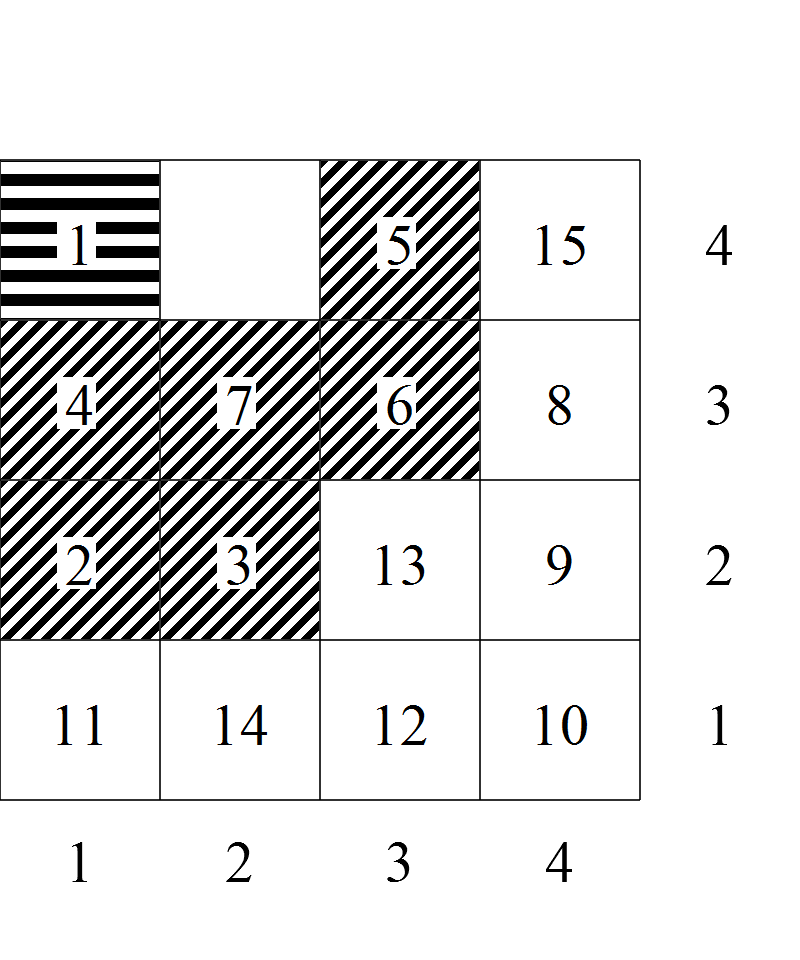
\includegraphics[width=\textwidth]{img/pre-solving-bsp-1.png}
    \caption{Das erste Bild}
    \label{fig:example:first:1st}
  \end{subfigure}
  \hfill
  \begin{subfigure}[t]{0.38\textwidth}
    \centering
    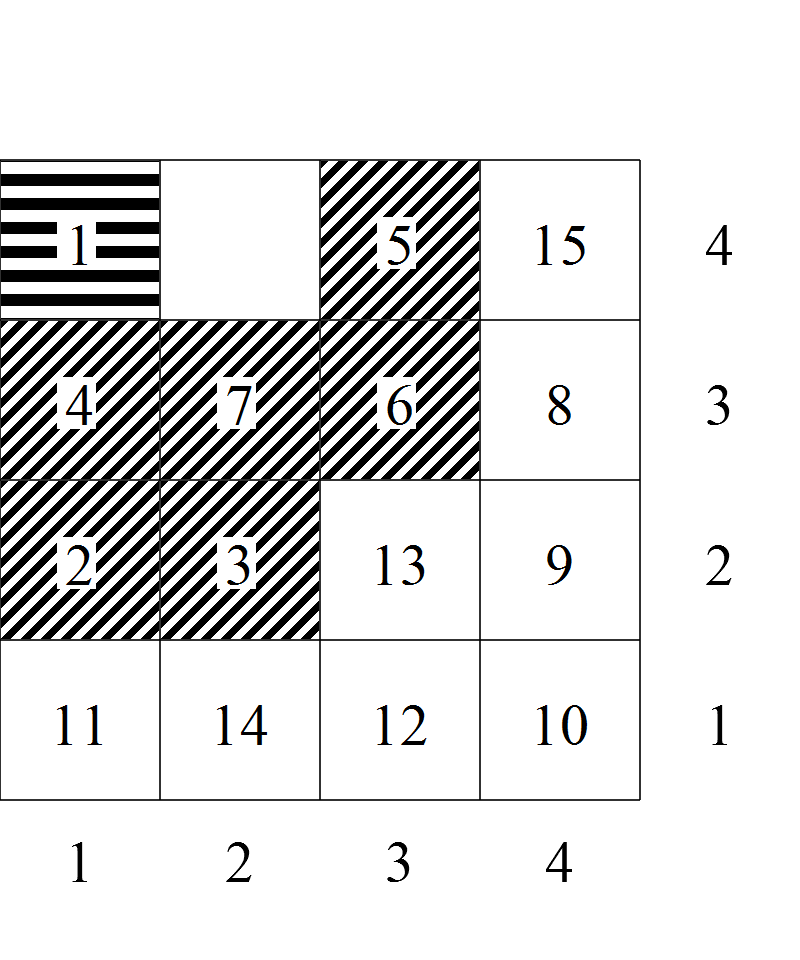
\includegraphics[width=\textwidth]{img/pre-solving-bsp-1.png}
    \caption{Das gleiche Bild, aber es könnte auch ein anderes sein!}
    \label{fig:example:first:2nd}
  \end{subfigure}

  \caption{Hier gibt es gleich zweimal was zu sehen.}
  \label{fig:example:first}
\end{figure}

Die ganze Abbilding hat das Label \texttt{fig:example:first} und kann dementsprechend mit
\texttt{\textbackslash{}ref\{fig:example:first\}} referenziert werden:
Abbildung~\ref{fig:example:first}.

Aber auch die enthaltenen \emph{Subfigures} haben ihre eigenen Label:
Abbildung~\ref{fig:example:first:1st} und Abbildung~\ref{fig:example:first:2nd}.
Diese Referenzen können auch in der Beschreibung der umgebenden Abbildung
benutzt werden um die Subabbildungen in Beziehung zueinander zu setzen.

\begin{figure}[htp]
  \centering
  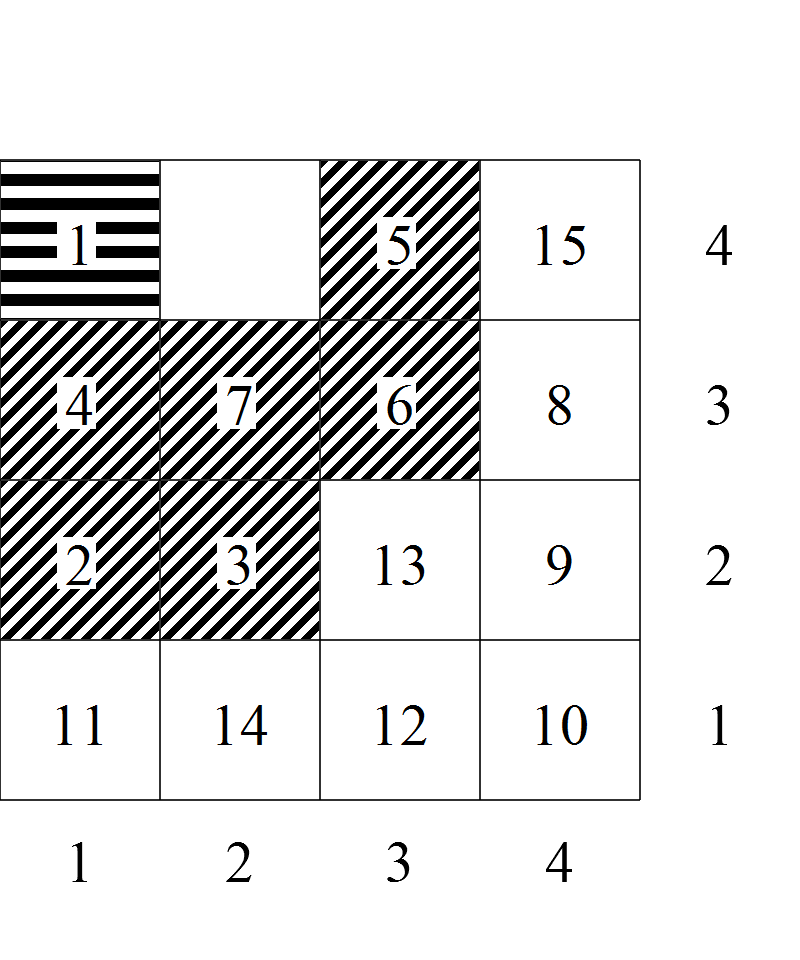
\includegraphics[width=0.3\textwidth]{img/pre-solving-bsp-1.png}
  \caption{Ein einzelnes Bild kann auch eingebunden werden...}
  \label{fig:einzeln}
\end{figure}


\paragraph{Bildformate}

Für Abbildungen~\ref{fig:example:first} wird eine PNG-Graphik
in das Dokument eingebunden.
Jedoch sollten Vektorgraphiken (PDF/SVG) gegenüber Rastergraphiken (PNG,GIF,JPG)
bevorzugt werden, da der Drucker und andere Ausgabegeräte selbstständig eine
angemessene Skalierung vornehmen können.
